\section{Induktivitätsmessbrücke}
\label{sec:Induktivitätsmessbrücke}

\tikzset{circuit declare symbol = AC source}
\tikzset{AC source IEC graphic/.style={
    circuit symbol lines,
    circuit symbol size=width 2 height 2,
    shape=generic circle IEC,
    /pgf/generic circle IEC/before background={
    \pgfpathmoveto{\pgfpoint{-0.8pt}{0pt}}
    \pgfpathsine{\pgfpoint{0.4pt}{0.4pt}}
    \pgfpathcosine{\pgfpoint{0.4pt}{-0.4pt}}
    \pgfpathsine{\pgfpoint{0.4pt}{-0.4pt}}
    \pgfpathcosine{\pgfpoint{0.4pt}{0.4pt}}
    \pgfusepath{stroke}
    },
    transform shape, draw
  }
}
\tikzset{circuit ee IEC/.append style=
  {set AC source graphic = AC source IEC graphic}
}

\subsection{Durchführung}
\label{subsec:Durchführung}

Die Induktivitätsmessbrücke ist der Kapazitätsmessbrücke 
sehr ähnlich, siehe Abbildung 6.

\begin{figure}
    \centering
    \begin{tikzpicture}[circuit ee IEC, font=\sffamily]
    \draw (0,0) to [AC source](0,-8);
    \draw (0,0) -- (3,0);
    \draw (3,0) -- (3, -1);
    \node[contact] at (3,-1) {};
    \draw (1.5, -1) -- (4.5, -1);
    \draw (1.5,-1) to [inductor={info={L$\mathsf{_{x}}$},info'={$\mathsf{_{}}$}}] (1.5,-2.5);
    \draw (1.5, -2.5) to [resistor={info={$R_x$}}] (1.5, -4);
    \draw (1.5,-4) to [inductor={info={L$\mathsf{_{2}}$},info'={$\mathsf{_{}}$}}] (1.5,-5.5);
    \draw (1.5, -5.5) to  [resistor={adjustable={info={$\mathsf{_{}}$}}, info'={R$\mathsf{_{2}}$}}] (1.5,-7);
    \draw (4.5, -1) to [resistor={info={$R_3$ \\ $R_4$}}] (4.5, -7);
    \node[scale=0.7] at (3, -3.5) {zum Y-Eingang};
    \node[scale=0.7] at (3,-3.75) {des Oszillographen};
    \node[scale=0.7] at (3,-4.2) {$U_b$};
    \node[contact] at (1.5,-4) {};
    \node[contact] at (2.5, -4) {};
    \node[contact] at (3.5,-4) {};
    \draw (1.5, -4) -- (2.5, -4);
    \draw (3.5, -4) -- (4.4, -4);
    \draw (1.5, -7) -- (4.5, -7);
    \node[contact] at (3,-7) {};
    \draw (0, -8) -- (3,-8);
    \draw (3, -8) -- (3,-7);
    \end{tikzpicture}
    \caption{Induktivitätsmessbrücke}
    \label{fig:Induktivitätsmessbrücke}
\end{figure}

Der einzige Unterschied besteht darin, dass statt eines Kondensators
eine Spule bzw. eine RL - Kombination eingebaut worden ist, deren 
Werte ermittelt werden soll. Das Messverfahren läuft analog zu der
der Kapazitätsmessbrücke. Dabei wird diesmal $L_2$ zwei Mal variiert. 

\subsection{Auswertung}
\label{subsec:Auswertung}

\begin{figure}
  \centering
  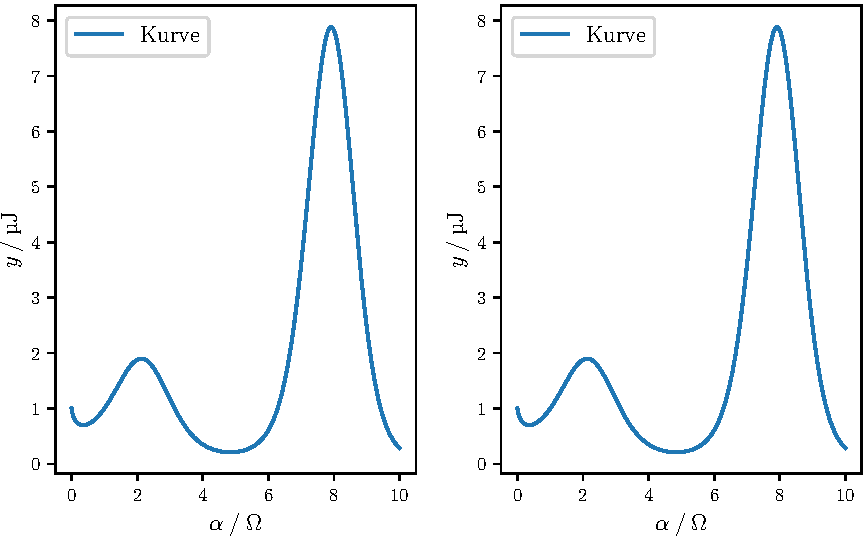
\includegraphics{plot.pdf}
  \caption{Plot.}
  \label{fig:plot}
\end{figure}